%-----------------------------------------------------------------------------
%
%               Template for sigplanconf LaTeX Class
%
% Name:         sigplanconf-template.tex
%
% Purpose:      A template for sigplanconf.cls, which is a LaTeX 2e class
%               file for SIGPLAN conference proceedings.
%
% Guide:        Refer to "Author's Guide to the ACM SIGPLAN Class,"
%               sigplanconf-guide.pdf
%
% Author:       Paul C. Anagnostopoulos
%               Windfall Software
%               978 371-2316
%               paul@windfall.com
%
% Created:      15 February 2005
%
%-----------------------------------------------------------------------------


%\documentclass[preprint]{sigplanconf}
\documentclass[10pt]{sigplanconf}

% The following \documentclass options may be useful:
%
% 10pt          To set in 10-point type instead of 9-point.
% 11pt          To set in 11-point type instead of 9-point.
% authoryear    To obtain author/year citation style instead of numeric.

\usepackage{yfonts}
\usepackage{amsmath}
\usepackage{amsthm}
\usepackage{amssymb}
%\usepackage{mathpartir}
\usepackage{hyperref}
\usepackage{url}
\usepackage{graphics}
\usepackage{graphicx}
\usepackage{wasysym}
\usepackage{harmony}
\usepackage{marvosym}
\usepackage{multirow}
\usepackage[usenames,dvipsnames]{xcolor}
\usepackage[charter]{mathdesign}
\usepackage{natbib}
\usepackage{xspace}
\usepackage[mathcal]{euscript}
\usepackage[linesnumbered,ruled]{algorithm2e}

\renewcommand{\UrlBreaks}{\do\/\do\a\do\b\do\c\do\d\do\e\do\f\do\g\do\h\do\i\do\j\do\k\do\l\do\m\do\n\do\o\do\p\do\q\do\r\do\s\do\t\do\u\do\v\do\w\do\x\do\y\do\z}

% ____________________________________________________________
% Listings Package Configuration
% \usepackage[scaled]{beramono}

%\renewcommand*\ttdefault{txtt}
\usepackage[T1]{fontenc}

% This Deep Tex Voodoo is from
%   <http://www.latex-community.org/forum/viewtopic.php?f=5&t=2072>
% It's purpose is to make \lstinline normal size, without affecting
% \lstinputlisting.  It seems to work but I have no idea how or why,
% and I rather hope never to learn.
%\makeatletter
%\lst@AddToHook{TextStyle}{\let\lst@basicstyle\ttfamily\normalsize}
%\makeatother

\begin{document}

\conferenceinfo{SIGBOVIK '18}{Pittsburgh, PA, USA}
\copyrightyear{2018}
\copyrightdata{}

\titlebanner{banner above paper title}        % These are ignored unless
\preprintfooter{short description of paper}   % 'preprint' option specified.

\title{
Transactional Memory Concurrency Verification with Landslide
%That `Boring' Stuff Was Part of the Title, BTW. \\
%So was that. And that, and this too. \\
%You got it all, right? \\
%Or Just, ``More Boring Crap about ITG'', for Short. \\
%Oh, That Was Also Part of the Title.
}
% \subtitle{\em The Randomly-Scoped Lambda Calculus}
% \subtitle{Subtitle Text, if any}

\authorinfo{Ben Blum}{}{bblum@cs.cmu.edu}

\maketitle

\begin{abstract}
Hardware transactional memory is a recently-introduced concurrent programming paradigm
%backed by a set of new instructions on recent x86 CPUs,
which allows programmers to elide locks for performance in low-contention workloads.
However,
%using this feature
it
comes at a cost in implementation complexity:
%programmers must support their
fast-path code must be accompanied by backup paths to handle transaction failure.

We extend Landslide, a popular stateless model checker,
with a concurrency model for transactional memory
and evaluate it on several real-world transactional
benchmarks and data structure implementations.
\end{abstract}

\category{D.1.3}{Programming Techniques}{Concurrent Programming}
\category{D.2.4}{Software Engineering}{Software/Program Verification}

\keywords
landslide terminal, baggage claim, ground transportation, ticketing

\section{Introduction}
\label{sec:intro}

Transactional Synchronization Extensions (TSX) \cite{transactional-memory}
is an instruction set extension for x86 CPUs which adds hardware-based transactional memory.
The processor uses its existing cache coherence algorithm to
check for memory conflicts with other cores while temporarily staging a sequence of memory accesses.
If no other CPU accesses the same memory during the transaction,
the access sequence is committed to main memory atomically (with respect to visibility to other CPUs).
Otherwise, the accesses are discarded, the CPU's local state is reverted, and the transaction returns a failure code.

This feature can be used to replace conventional locking in performance-critical concurrent programs.
When a concurrent workload accesses largely thread-local data,
or disjoint sections of a shared data structure,
the contention rate between threads is low,
and transactions will often succeed.
Compared to programs which use conventional locks,
which use bus-locking atomic accesses even in the fastest code path,
TSX provides substantial performance improvements in such programs \cite{htm-experience, htm-performance, htm-mario}.
However, the possibility of transaction failure introduces additional implementation complexity:
programmers must also provide a backup plan
to safely resolve contention between threads,
usually involving conventional synchronization.
These backup paths must coordinate not only with other backup paths
but also with other fast paths which another thread may begin after the original transaction failed,
which even in the simplest transactions requires complex synchronization sequences
\cite{htm-mario}.
This introduces an additional dimension of nondeterminism into an already concurrent program,
and moreover, because transaction failure is expected to be rare,
% だからこそ
obscure interleavings between failure paths are difficult to expose during testing.

This motivates the use of stateless model checking (MC) \cite{verisoft}
to comprehensively verify these transactional programs,
fast paths failure paths and all.
MC aims to force the system to execute all possible thread interleavings under a given test case,
exhaustively checking for bugs or verifying their absence in the corresponding state space.
Many such model checkers exist, varying in
interleaving granularity, memory analysis, types of programs checked, and search ordering strategy
\cite{chess,dbug-ssv,spin,inspect,r4,portend,samc,mcr,randomized-scheduler}.
This work builds upon Landslide \cite{landslide,quicksand,landslide-phdthesis},
a simulator-based tester which checks both user- and kernel-level programs
and incorporates data-race analysis \cite{tsan,fasttrack} to find new preemption points
at memory access granularity.
Our contributions are as follows:

\begin{enumerate}
	\item We extend Landslide's concurrency model to include transaction failure as an additional source of nondeterminism;
	\item We provide a proof sketch that our implementation matches TSX's execution semantics,
	\item We evaluate the extended Landslide on several transactional programs, analyzing both its bug-finding and verification performance.
\end{enumerate}

The paper is organized as follows.
Section \ref{sec:intro} introduces the problem domain and motivates our research.
The other sections state the rest of the paper.

%%%%%%%%%%%%%%%%%%%%%%%%%%%%%%%%%%%%%%%%%%%%%%%%%%%%%%%%%%%%%%%%%%%%%%%%%%%%%%%%

\section{Background}
\label{sec:background}

This section introduces the fundamental concepts and prior work
in both hardware transactional memory and stateless model checking,
which we propose to combine.

{\bf Hardware transactional memory.}
TSX was supported on consumer hardware for the first time by Intel's Haswell architecture \cite{htm-haswell},
which extends the x86 instruction set to provide
{\tt xbegin}, {\tt xend}, and {\tt xabort} for beginning, committing, and aborting
transactions, respectively.
Higher-level programming languages or compilers may offer libraries or intrinsics to access these instructions;
for C and C++ GCC provides intrinsics named {\tt \_xbegin()} and so on \cite{htm-gcc}.
Figure~\ref{fig:htm-example} shows an example program using TSX to synchronize access to a shared counter,
including a failure path which defaults to a conventional lock.
This example actually has a bug, which we will discuss in the next section;
the reader is encouraged to try to spot it before then.
Several related works formally prove the correctness of transactional memory {\em implementations}
\cite{specifying-verifying-tm,tm-correctness,tm-completeness,mc-tm-with-spin},
but verifying the client programs written to use transactions remains an open problem.

\begin{figure}[t]
	\begin{center}
		\begin{tabular}{ll}
		%\texttt{void count() \{} \\
		%\texttt{~~~~for (int i = 0; i < 1000; i++) \{} \\
		1 & \texttt{if ((status = \_xbegin()) == SUCCESS) \{} \\
		2 & \texttt{~~~~x++;} \\
		3 & \texttt{~~~~\_xend();} \\
		4 & \texttt{\} else \{} \\
		5 & \texttt{~~~~mutex\_lock(\&m);} \\
		6 & \texttt{~~~~x++;} \\
		7 & \texttt{~~~~mutex\_unlock(\&m);} \\
		8 & \texttt{\}} \\
		%\texttt{~~~~\}} \\
		%\texttt{\}} \\
		\end{tabular}
	\end{center}
	\caption{Example transactional program.
		%The example {\tt count} routine from Figure~\ref{fig:mutex}, rewritten to use HTM.
		If the
		%transaction in the
		top branch aborts,
		%whether from a memory conflict or random system interrupt,
		%from the programmer's intention,
		execution will revert to the return of {\tt \_xbegin()}
		%{\tt status} will be assigned an error code
		and control will drop into the {\tt else} branch.
		The programmer can then use explicit synchronization
		%, such as a mutex,
		to resolve the conflict.}
	\label{fig:htm-example}
\end{figure}

Under software transactional memory (STM) \cite{stm-pldi06},
memory conflicts with other threads are the only reason for transaction failure
(apart from programmer-supplied explicit aborts);
hence, depending on program semantics, some transactions may be guaranteed to succeed.
However, hardware implementations (HTM) may also fail transactions
for several other reasons such as random system interrupts or exhausting the CPU's cache capacity.
Because timer interrupts can in principle occur at any moment,
and with arbitrary frequency (observable by the program, perhaps as a result of a heavily-loaded system),
in this paper we will simplify the failure model by saying that HTM transactions can fail for any reason.
We defer discussion of programs which distinguish the reason for aborts through the failure code to Section~\ref{sec:warpzone}.

{\bf Stateless model checking.}
Model checking (MC) \cite{verisoft} is a testing technique for systematically executing and verifying
the possible thread interleavings of a concurrent program.
The main research challenge is to cope with exponential explosion of the state space,
which is $O(n^k)$ for a program with $n$ operations and $k$ threads.
Some {\em stateful} MCs explicitly store and compare all visited states of the program being tested \cite{spin},
which both keeps track of test coverage
and allows identifying identical states to avoid testing redundant interleavings.
%
By contrast, {\em stateless} MC (henceforth abbreviated simply as MC)
stores only the current sequence of execution events to avoid a prohibitive memory footprint.
Reduction algorithms \cite{dpor,optimal-dpor,satcheck,mcr,mcr,tsopso}
can then analyze the memory accesses in that sequence to identify
interleavings observationally-equivalent under Mazurkiewicz trace theory \cite{mazurkiewicz} and hence safe to skip.
The resulting state spaces are still exponentially-sized,
but only in the number of conflicting operations rather than all operations.
Of these, Landslide uses Dynamic Partial Order Reduction (DPOR) \cite{dpor} to prune its state spaces.

MCs may instrument programs to introduce thread switches at varying granularity, which affects the number of operations $n$.
%The number of operations depends on how finely-grained the MC instruments the program to introduce thread switches.
Some target distributed systems, instrumenting only message-passing events \cite{modist};
some run multithreaded programs natively, instrumenting only the pthread API for performance \cite{dbug-ssv};
and some insert compiler instrumentation on statically-identified memory accesses \cite{chess,inspect}.
Landslide traces every memory access through the use of a simulated environment \cite{bochs},
which is important for identifying data races to use as new preemption points \cite{fasttrack,djit,quicksand},
as well as for identifying when a memory conflict may cause transaction aborts.
With regard to checking for bugs,
the ``model'' the name refers to being checked may be
an external formal specification,
the program's own internal consistency checks,
or a set of expected properties encoded in the tool itself.
Landslide uses the latter two cases, checking for assertion failures
as well as deadlocks, use-after-frees, and segfaults.
For this work we also detect use of {\tt xend} outside of a transaction as a bug.

%%%%%%%%%%%%%%%%%%%%%%%%%%%%%%%%%%%%%%%%%%%%%%%%%%%%%%%%%%%%%%%%%%%%%%%%%%%%%%%%

\section{Design}
\label{sec:design}

This section presents our formalization of transactional memory in Landslide's framework of thread concurrency.
We make two major simplifications:
simulating transaction aborts as failure injections,
and treating transaction atomicity as a global mutex during data-race analysis;
and provide corresponding equivalence proofs.

{\bf Notation.} Let $I = TN_1@L_1, TN_2@L_2, ... TN_n@L_n$,
with $N_i$ a thread ID and $L_i$ a code line number,
denote the execution sequence of a program as it runs according to the specified thread interleaving.%
\footnote{This serialization of concurrent execution is told from the perspective of main memory
and hence assumes sequential consistency.
For discussion of relaxed memory models refer to Section~\ref{sec:warpzone}.}

\subsection{Example}

Consider again the program in Figure~\ref{fig:htm-example}.
Note that the C-style {\tt x++} operations, when compiled into assembly,
results in multiple memory accesses which can be interleaved with other threads.
\[
\begin{tabular}{ll}
	$2a$ & \texttt{temp <- x;} \\
	$2b$ & \texttt{temp <- temp + 1;} \\
	$2c$ & \texttt{x <- temp;} \\
\end{tabular}
\]

\newcommand\hilight[2]{\color{#1}#2\color{black}}
\definecolor{orange}{RGB}{192,96,0}
\definecolor{olivegreen}{RGB}{0,127,0}
\definecolor{brickred}{RGB}{192,0,0}
\definecolor{commentblue}{RGB}{0,0,192}
\definecolor{black}{RGB}{0,0,0}
%\definecolor{lavender}{RGB}{238,85,238}
%\definecolor{seafoam}{RGB}{85,238,102}
%\definecolor{salmon}{RGB}{238,102,85} % ee6655

\definecolor{lavender}{RGB}{102,65,208} % (?? i don't know what happened here anymore but it looks good)
\definecolor{seafoam}{RGB}{65,178,76} % * 3/4
\definecolor{salmon}{RGB}{208,89,74} % * 7/8

% T1 T2 T3 but latex doesn't allow #s in cmd names
\newcommand\ti{\ensuremath{\hilight{lavender}{\mathbf{T1}}}\xspace}
\newcommand\tj{\ensuremath{\hilight{seafoam}{\mathbf{T2}}}\xspace}
\newcommand\tk{\ensuremath{\hilight{salmon}{\mathbf{T3}}}\xspace}

\newcommand\tiat[1]{\ensuremath{\hilight{lavender}{\mathbf{T1}@#1}}\xspace}
\newcommand\tjat[1]{\ensuremath{\hilight{seafoam}{\mathbf{T2}@#1}}\xspace}
\newcommand\tkat[1]{\ensuremath{\hilight{salmon}{\mathbf{T3}@#1}}\xspace}

If these instructions from the {\tt x++} in the transaction are preempted,
with another thread's access to {\tt x} interleaved in between,
the transaction will abort.
So, the interleaving
\[
	\tiat{1}, \tiat{2a}, \tiat{2b}, \tjat{1}, \tjat{2}, \tjat{3}, \tiat{2c}, \tiat{3}
\]
or, henceforth abbreviated for clarity:
\[
	\tiat{1-2b}, \tjat{1-3}, \tiat{2c-3}
\]
is not possible; rather, \ti will fall into the backup path:
\[
	\tiat{1-2b}, \tjat{1-3}, \tiat{4-7}
\]
However, the {\tt x++} operation from the failure path (correspondingly $6a$, $6b$, $6c$)
{\em can} be thusly separated with conflicting accesses interleaved in between,
since the mutex only protects the failure path against other failure paths,
but not against the transaction itself.
So (assuming {\tt x} is intended to be a precise counter rather than a sloppy one),
%losing one of the increments to which constitutes a bug),
we observe a bug in the following interleaving.%
\footnote{Note also that this bug requires either at least 3 threads or at least 2 iterations between 2 threads to expose;
this highlights MC's dependence on its test cases to produce meaningful state spaces in the first place.}
\[
	\tiat{1-2b}, \tjat{1-3}, \tiat{4-6b}, \tkat{1-3}, \tiat{6c-7}
\]
Prior work \cite{htm-mario} proposed the idiom shown in Figure~\ref{fig:htm-fixed}
to exclude this family of interleavings,
showing that correctly synchronizing even the simplest transactions may be surprisingly difficult or complex.
%further motivating our research.

\begin{figure}[t]
	\begin{center}
		\begin{tabular}{ll}
		%\texttt{void count() \{} \\
		%\texttt{~~~~for (int i = 0; i < 1000; i++) \{} \\
		  & \texttt{prevent\_transactions = false;} \\
		\\
		0 & \texttt{while (prevent\_transactions) continue;} \\
		1 & \texttt{if ((status = \_xbegin()) == SUCCESS) \{} \\
		2 & \texttt{~~~~if (prevent\_transactions)} \\
		3 & \texttt{~~~~~~~~\_xabort();} \\
		4 & \texttt{~~~~x++;} \\
		5 & \texttt{~~~~\_xend();} \\
		6 & \texttt{\} else \{} \\
		7 & \texttt{~~~~mutex\_lock(\&m);} \\
		8 & \texttt{~~~~prevent\_transactions = true;} \\
		9 & \texttt{~~~~x++;} \\
		A & \texttt{~~~~prevent\_transactions = false;} \\
		B & \texttt{~~~~mutex\_unlock(\&m);} \\
		C & \texttt{\}} \\
		%\texttt{~~~~\}} \\
		%\texttt{\}} \\
		\end{tabular}
	\end{center}
	\caption{Variant of the program in Figure~\ref{fig:htm-example},
		with additional synchronization to protect the failure path from the transactional path.
		The optional line 0 serves to prevent a cascade of failure paths
		for the sake of performance
		by allowing threads to wait until transacting is safe again.}
	\label{fig:htm-fixed}
\end{figure}

\subsection{Modeling Transaction Failure}

Left unstated in interleavings such as $\tiat{1-2c}, \tjat{1-3}, \tiat{4-7}$%
\footnote{For the sake of example I reorder \ti's write to {\tt x} before \tj's part here.}
are HTM's execution semantics, namely:
\begin{enumerate}
	\item any modifications to shared state (such as $2c$) by \ti are not visible to \tj during its execution,
		despite \tj being executed afterwards, and
	\item all local and global state changes by \ti between lines $1$ and $2c$ are discarded when jumping to line $4$.
\end{enumerate}
% there shouldbe a better word than 'requires' here.. benefits from.. "the point of it is"..
While use of TSX in production requires the performance advantage
of temporarily staging such accesses in local CPU cache,
model checking such programs need be concerned only with the program's {\em observable} behaviours.
We claim that MCing the interleaving $\tiat{1}, \tjat{1-3}, \tiat{4-7}$
is an equivalent verification as MCing the one above;
in fact, this interleaving suffices to check
all observable behaviours
of all interleavings
of all subsets of $\tjat{1-3}$
with all subsets of $\tiat{2a-2c}$,
whether they share a memory conflict or not.
Stated formally:

\renewcommand\proofname{Proof Sketch}
\newtheorem{lemma}{Lemma}
\newtheorem{theorem}{Theorem}
\newtheorem{definition}{Definition}

\newcommand\tii{\ensuremath{\hilight{lavender}{\mathbf{Ti}}}\xspace}
\newcommand\tjj{\ensuremath{\hilight{seafoam}{\mathbf{Tj}}}\xspace}
\newcommand\tkk{\ensuremath{\hilight{salmon}{\mathbf{Tk}}}\xspace}

\newcommand\tiiat[1]{\ensuremath{\hilight{lavender}{\mathbf{Ti}@#1}}\xspace}
\newcommand\tjjat[1]{\ensuremath{\hilight{seafoam} {\mathbf{Tj}@#1}}\xspace}
\newcommand\tkkat[1]{\ensuremath{\hilight{salmon}  {\mathbf{Tk}@#1}}\xspace}

\newcommand\llama[1]{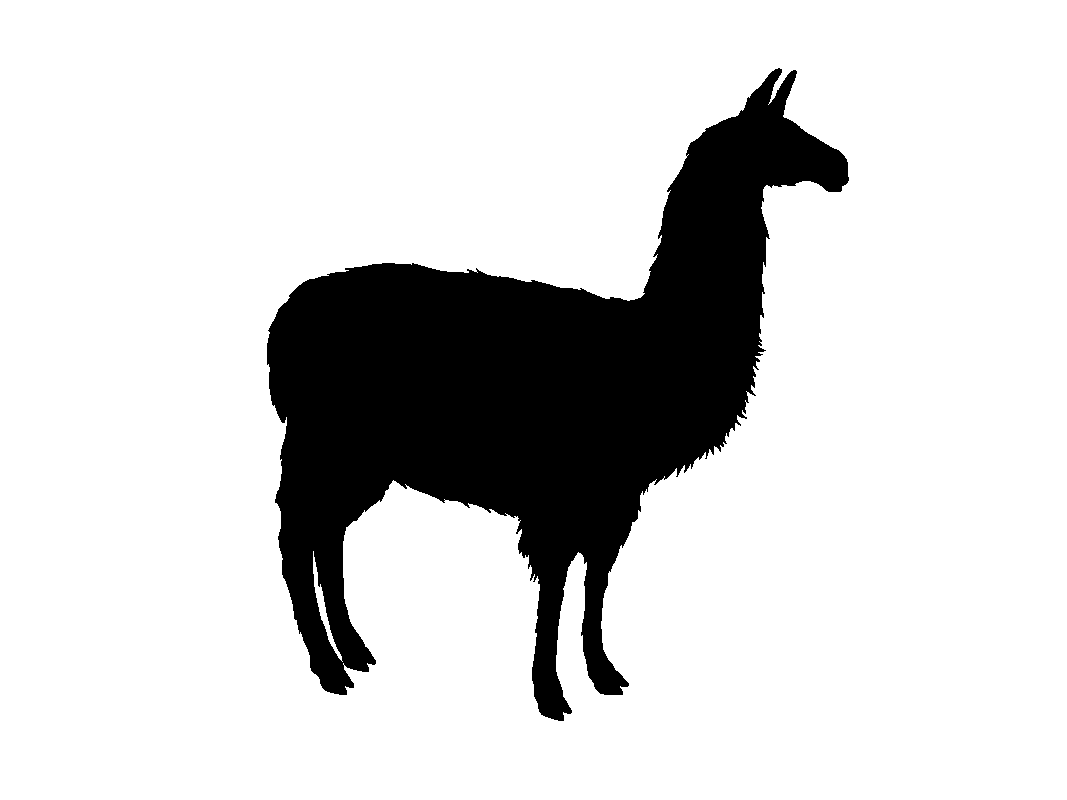
\includegraphics[width=#1]{llama.pdf}}
\newcommand\llitem{\item[\raisebox{-0.15em}{\llama{1.2em}}]}

\begin{lemma}[Equivalence of Aborts]
	\label{lem:equiv}
	Let:
	\begin{itemize}
		\item $\tiiat{\alpha}$ be an HTM begin operation,
		\item $\tiiat{\beta_1}\dots\tiiat{\beta_n}$ be the transaction body (with $\beta_n$ the HTM end call),
		\item $\tiiat{\phi_1}\dots\tiiat{\phi_m}$ be the failure path, and
		\item $\tiiat{\omega_1}\dots\tiiat{\omega_l}$ be the subsequent code executed unconditionally.%
			\footnote{Arbitrary code may not be structured to distinguish these as nicely as in our examples;
			e.g., more code may exist in the success branch after {\tt \_xend()};
			such would be considered part of $\omega$ here.}
	\end{itemize}
	Then, for any interleaving prefix%
	\footnote{Without loss of generality: for any number of other threads \tjj/\tkk,
	and for any number of thread switches away from \tii during the transaction.}
	\[
	\begin{tabular}{c}
		$\tiiat{\alpha},\tiiat{\beta_1}\dots\tiiat{\beta_b},$\\
		$\tjjat{\gamma_1}\dots\tjjat{\gamma_j},$ \\
		$\tkkat{\kappa_1}\dots\tkkat{\kappa_k},$ \\
		$\tiiat{\beta_{b+1}}$ % $\dots\tiiat{\beta_{n-1}}$ -- excluded bc might abort
	\end{tabular}
	\]
	with $b<n$, $j \ne i$, $k \ne i$, etc., either:
	\begin{enumerate}
		\item $\tiiat{\alpha},\tjjat{\gamma_1}\dots\tjjat{\gamma_j},\tkkat{\kappa_1}\dots\tkkat{\kappa_k},\tiiat{\phi_1}\dots$
			(conflicting case), or
		\item $\tiiat{\alpha},\tiiat{\beta_1}\dots\tiiat{\beta_b}\dots\tiiat{\beta_n},\tjjat{\gamma_1}\dots\tjjat{\gamma_j},$ \\
			$\tkkat{\kappa_1}\dots\tkkat{\kappa_k}$
			(independent case)
	\end{enumerate}
	exists and is observationally equivalent.
\end{lemma}

\begin{proof}
	We case on whether the operations by \tjj and/or \tkk have any memory conflicts (read/write or write/write)
	with $\tiiat{\beta_1}\dots\tiiat{\beta_n}$.
	If so, then the hardware will abort \tii's transaction, discarding the effects of $\tiiat{\beta_1}\dots\tiiat{\beta_n}$
	and jumping to $\tiiat{\phi_1}$,
	satisfying case 1.
	Otherwise, by DPOR's definition of transition dependence \cite{dpor,landslide-phdthesis},
	$\tiiat{\beta_{b+1}}\dots\tiiat{\beta_n}$ is independent with the transitions of \tjj and \tkk,
	may be successfully executed until transaction commit,
	and reordering them produces an equivalent interleaving,
	satisfying case 2.
\end{proof}

The second part of our claim follows naturally.

\begin{theorem}[Atomicity of Transactions]
	\label{thm:atom}
	For any state space $S$ of a transactionally-concurrent program,
	an equivalent state space exists in which all transactions are either executed atomically or aborted immediately.
\end{theorem}

\begin{proof}
	For every $I \in S$ with $\tiiat{\alpha},\tiiat{\beta_1}\dots\tiiat{\beta_b},$ $\tjjat{\dots},\tkkat{\dots},\tiiat{\beta_{b+1}} \in I$,
	apply Lemma~\ref{lem:equiv} to obtain an equivalent interleaving $I'$ satisfying the theorem condition.
	The resulting $S'$ can then be MCed without ever simulating HTM rollbacks.
\end{proof}

\subsection{Memory Access Analysis}

Next, we address the memory accesses within transactions with regard to data-race analysis.
From Theorem~\ref{thm:atom} we have that the body of all transactions may be executed atomically within the MC environment.
While they may interleave within other non-transactional sequences,
no other operations (whether transactional or not) will interrupt them.
We claim this level of atomicity is equivalent to that provided by a global lock,
and hence abstracting it as such in Landslide's data-race analysis is sound.

Let $\tiiat{\mu},\tjjat{\nu}$ be a pair of memory accesses to the same address, at least one a write,
in some transactional execution $I$ normalized under Lemma~\ref{lem:equiv}.
Then let $\mathsf{lockify}_m(\tkkat{L})$ denote a function over instructions in $I$,
which replaces $\tkkat{L}$ with $\tkkat{\mathsf{lock}(m)}$ if $L$ is a successful HTM begin,
with a no-op if $L$ is a transaction abort,
or with $\tkkat{\mathsf{unlock}(m)}$ if $L$ is an HTM end,
or no replacement otherwise.
Finally, let $I' = \exists m. \mathsf{lockify}_m(I)$,
the execution with the boundaries of all successful transactions replaced by an abstract global lock.
Lemma~\ref{lem:equiv} guarantees mutual exclusion of $m$.

\begin{theorem}[Transactions are a Global Lock]
	$\tiiat{\mu},\tjjat{\nu}$ is a data race in $I$ iff it is a data race in $I'$.
\end{theorem}

\begin{proof}
We prove one case for each variant definiton for data races supported in Landslide \cite{quicksand}.
For each, we semiformally state what it means to race in an execution with synchronizing HTM instructions.

\begin{itemize}
	\item {\bf Limited Happens-Before.}
		Under this definition, to be a data race in $I$ they must be reorderable at instruction granularity
		\cite{tsan,hybriddatarace}.
		\begin{itemize}
			\llitem $I \Rightarrow I'$:
				If $\tiiat{\mu},\tjjat{\nu}$ race in $I$,
				then they cannot both be in successful transactions,
				or else placing \tiiat{\mu} within the boundaries of \tjjat{\nu}'s transaction
				would cause the latter to abort, invalidating \tjjat{\nu}, or vice versa.
				Hence they will not both hold $m$ in $I'$.
				Otherwise their lock-sets and DPOR dependence relation remain unchanged.
			\llitem $I' \Rightarrow I$:
				If $\tiiat{\mu},\tjjat{\nu}$ race in $I'$,
				both corresponding threads cannot hold $m$;
				WLOG let $\tii$ not hold $m$ during $\tiiat{\mu}$.
				Then in $I$, $\tiiat{\mu}$ is not in a transaction.
				With the remainder of their lock-sets still disjoint,
				and still not DPOR-dependent, $\tjjat{\nu}$ (or its containing transaction)
				can then be reordered directly before or after $\tiiat{\mu}$.
		\end{itemize}
	\item {\bf Pure Happens-Before.}
		WLOG fix $\tiiat{\mu} \prec \tjjat{\nu} \in I$.
		Then under this definition, to be a data race in $I$ there must be no pair of synchronizing instructions
		$\tiiat{\epsilon}$ (a release edge) and $\tjjat{\chi}$ (an acquire edge) such that
		\[
			\tiiat{\mu} \prec \tiiat{\epsilon} \prec \tjjat{\chi} \prec \tjjat{\nu} \in I
		\]
		to update the vector clock epoch between \tiiat{\mu} and \tjjat{\nu} \cite{djit,fasttrack}.
		\begin{itemize}
			\llitem $I \Rightarrow I'$:
				If $\tiiat{\mu},\tjjat{\nu}$ race in $I$,
				then they cannot both be in successful transactions,
				or else Lemma~\ref{lem:equiv} normalization would provide
				the corresponding HTM end and begin for $\tiiat{\epsilon}$ and $\tjjat{\chi}$ respectively.
				Hence there will be no unlock/lock pair on $m$ in $I'$ to satisfy the above sequence.
			\llitem $I' \Rightarrow I$:
				If $\tiiat{\mu},\tjjat{\nu}$ race in $I'$,
				then they cannot both hold $m$,
				or else $\mathsf{lockify}_m$ would provide the corresponding
				unlock and lock for $\tiiat{\epsilon}$ and $\tjjat{\chi}$ respectively.
				Hence there will be no HTM end/begin pair in $I$ to satisfy the above sequence.
		\end{itemize}
		%In both cases $I$ and $I'$ otherwise have the same synchronizing instructions.
\end{itemize}
Hence, data-race analysis is sound when transaction boundaries are replaced by an abstract global lock.
\end{proof}

\subsection{Implementation}

Our implementation of HTM has been incorporated by the Landslide maintainers upstream.
The repository is available open-source at \url{https://github.com/bblum/landslide}.
Programs should be ported to the Pebbles userland \cite{thrlib,kspec},
their use of compiler HTM intrinsics should be replaced with the Landslide stubs provided in {\tt 410user/inc/htm.h},
and HTM nondeterminism can then be enabled with the {\tt -X} command-line flag.
We have also extended its Iterative Deepening implementation \cite{quicksand}
with an option ({\tt -M} flag) to
to optimize for completion time by prioritizing the maximal state space job and cancelling all others,
while maintaining its soundness guarantee,
which we will use in our evaluation.
All test cases therein are also available in the repository linked above.
%Several example tests are also provided:
%{\tt htm1} demonstrates the bug in Figure~\ref{fig:htm-example},
%and {\tt htm2} demonstrates Figure~\ref{fig:htm-fixed}'s fix.

%%%%%%%%%%%%%%%%%%%%%%%%%%%%%%%%%%%%%%%%%%%%%%%%%%%%%%%%%%%%%%%%%%%%%%%%%%%%%%%%

\section{Evaluation}

\definecolor{darkcyan}{RGB}{0,128,128}
\definecolor{lime}{RGB}{48,128,0}
\definecolor{pinkish}{RGB}{128,34,102} % ff4488
\definecolor{brownish}{RGB}{128,96,0}
\newcommand\ETA[1]{\hilight{brownish}{{\em #1}}\xspace}
\newcommand\cpu[1]{\hilight{darkcyan}{{#1}}\xspace}
\newcommand\wtm[1]{\hilight{lime}{{#1}}\xspace}
\newcommand\ints[1]{\hilight{pinkish}{{#1}}\xspace}

\begin{table*}[t]
	\begin{center}
		% TODO: highlight the winning statistic for each test
	\begin{tabular}{cc||r|r|r||r|r|r|r}
			&	&\multicolumn{3}{c||}{\bf Quicksand mode}&\multicolumn{4}{c}{{\bf Maximal state space mode} ({\tt -M})} \\
		\bf buggy test	& \bf params&\cpu{\bf cpu (s)}&\wtm{\bf wall (s)}&\ints{\bf int's}&\cpu{\bf cpu (s)}&\wtm{\bf wall (s)}&\ints{\bf int's}& \ETA{\bf SS size (est.)} \\
		\hline
		\hline
		{\tt htm1}
			& 2,1	&\cpu{  45.78}&\wtm{9.70}&\ints{21}& \cpu{9.47}& \wtm{6.40}& \ints{21	}& \ETA{213} \\
		(assertion)
			& 2,2	&\cpu{  84.14}&\wtm{13.59}&\ints{33}& \cpu{10.39}& \wtm{7.70}& \ints{49	}& \ETA{1536} \\
			& 2,3	&\cpu{ 131.91}&\wtm{20.44}&\ints{73}& \cpu{12.83}& \wtm{9.67}& \ints{113	}& \ETA{10752} \\
			& 2,4	&\cpu{ 255.75}&\wtm{37.56}&\ints{257}& \cpu{18.63}& \wtm{15.86}& \ints{257	}& \ETA{73728} \\
		\cline{2-9}
			& 3,1	&\cpu{ 114.06}&\wtm{17.45}&\ints{15}& \cpu{9.50}& \wtm{6.79}& \ints{21	}& \ETA{13653} \\
			& 3,2	&\cpu{ 109.60}&\wtm{26.16}&\ints{49}& \cpu{10.72}& \wtm{7.97}& \ints{49	}& \ETA{393216} \\
			& 3,3	&\cpu{ 124.80}&\wtm{20.40}&\ints{73}& \cpu{13.84}& \wtm{11.01}& \ints{113	}& \ETA{11010048} \\
			& 3,4	&\cpu{ 227.49}&\wtm{35.15}&\ints{161}& \cpu{31.37}& \wtm{28.53}& \ints{257	}& \ETA{301989888} \\
		\cline{2-9}
			& 4,1	&\cpu{ 53.08}&\wtm{9.79}&\ints{15}& \cpu{9.82}& \wtm{7.00}& \ints{21	}& \ETA{873813} \\
			& 4,2	&\cpu{117.07}&\wtm{19.09}&\ints{33}& \cpu{11.54}& \wtm{8.55}& \ints{49	}& \ETA{100663296} \\
		\hline
		{\tt swapbug}
			& 2,1	&\cpu{ 70.95}&\wtm{13.45}&\ints{16}& \cpu{38.96}& \wtm{13.15}& \ints{109	}& \ETA{194} \\
		(deadlock)
			& 2,2	&\cpu{ 107.28}&\wtm{17.45}&\ints{146}& \cpu{44.73}& \wtm{19.47}& \ints{281	}& \ETA{1620} \\
			& 2,3	&\cpu{ 280.05}&\wtm{38.70}&\ints{352}& \cpu{60.30}& \wtm{35.55}& \ints{718	}& \ETA{12748} \\
			& 2,4	&\cpu{ 617.94}&\wtm{81.50}&\ints{834}& \cpu{108.58}& \wtm{82.60}& \ints{1820	}& \ETA{97823} \\
		\cline{2-9}
			& 3,1	&\cpu{1275.04}&\wtm{163.42}&\ints{771}&\ETA{>30m}&\ETA{>30m}&\ETA{unk.}& \ETA{184984} \\
			& 3,2	&\ETA{>30m}&\ETA{>30m}&\ETA{unk.}&\ETA{>30m}&\ETA{>30m}&\ETA{unk.}& \ETA{3099225} \\
		% whoops, this was with the dumb lock ordering
		%	& 3,1	& 11.19	& 3.46	& 9	& 3.13	& 3.13	& 9	& 432 \\
		%	& 3,2	& 12.41	& 3.76	& 19	& 3.33	& 3.33	& 19	& 5832 \\
		%	& 3,3	& 15.77	& 4.58	& 41	& 3.95	& 3.95	& 41	& 77759 \\
		%	& 3,4	& 24.82	& 6.85	& 89	& 5.20	& 5.20	& 89	& 1026431 \\
		%\cline{2-9}
		%	& 4,1	& 702.33& 98.06	& 361	& 90.94	& 64.27	& 1607	& 138758 \\
		%	& 4,2	&9738.43&1257.20& 3023	& 674.87& 650.58& 16511	& 13755188 \\
	\end{tabular}
	\end{center}
	\caption{Landslide's bug-finding performance on various test configurations.
		Quicksand's workqueue approach optimized for fast bug-finding
		is compared against our maximum-state-space-prioritizing approach for fast verification.
		For each, we list the CPU-time and wall-clock time %(both in seconds)
		elapsed, %until the bug was found,
		plus the number of interleavings of the ultimately buggy state space tested,
		before the bug was found.
		Lastly, Landslide's state space size estimation \cite{estimation},
		though approximate at best,
		confers a sense of the exponential explosion.
	}
	\label{tab:buges}
\end{table*}

To the best of our knowledge, this is the first work to test transactional programs in a model-checking environment,
%To the best of the author's knowledge, Landslide is the first MC to check transactional concurrency,
so no other MC State-of-the-Art%
\footnote{The author's DJ name.}
exists to compare to in controlled experiments.
Nevertheless, we pose the following evaluation questions.

\begin{enumerate}
	\item How quickly does Landslide find bugs in incorrect transactional programs of varying sizes?
	\item How quickly does Landslide verify correct transactional programs of varying sizes?
	%\item Does Landslide find any previously-unknown bugs in real-world transactional code?
	\item By the way, should MC research papers quantify variance in their CPU-time performance experiments?
\end{enumerate}

Our evaluation suite comprises several hand-written unit tests
and \cite{htm-mario}'s microbenchmarks and transactional AVL tree and separate-chaining hashmap,
as follows.

\begin{itemize}
	\item {\tt htm1}: The bug from Figure~\ref{fig:htm-example}. %(assertion failure on {\tt count}).
	\item {\tt htm2}: The fixed version as in Figure~\ref{fig:htm-fixed}.
	\item {\tt counter}: Microbenchmark version of {\tt htm2} which replaces the complex failure path with a simple {\tt xadd}.
	\item {\tt swap}: Microbenchmark that swaps values in an array.
	\item {\tt swapbug}: {\tt swap} modified to introduce circular locking in the failure path. %(deadlock).
	\item {\tt map\_basic}: Concurrent insertion test for the separate-chaining hashmap.
	\item {\tt map\_basicer}: {\tt map\_basic} modified with a larger initial size to skip the resizing step.
		% TODO more
\end{itemize}

The notation {\tt testname}$(K,N)$ will denote a test configuration of $K$ threads, each running $N$ iterations of the test logic.
All tests were run on an 8-core 2.7GHz Core i7 with 32 GB RAM.

\subsection{Bugs}

Table~\ref{tab:buges}
presents our bug-finding results.
We configured Landslide to run the Quicksand algorithm \cite{quicksand}
% this note obsolete since swapbug was fixed and ends at 3,2
%\footnote{This was necessary in {\tt swapbug}s (4,1) and (4,2) to trigger a switch to the buggy state space.}
shown left,
as well as to prioritize the maximal state space as discussed above,
shown right,
each with a time limit of 30 minutes.
We make two observations/conclusions:
\begin{itemize}
	\item The multiplicative factor in bug-finding speed (2-4x, eyeballing) is generally smaller
		than that of the total number of interleavings (10-100x)
		as the test parameters increase.
		In other words,
		should they exist,
		Landslide find bugs reasonably quickly in these transactional programs
		despite prohibitive exponential explosion in total state space size.
	%\item Despite Quicksand's ability to optimize for finding bugs in overall smaller state spaces,
	%	this does not correlate with better CPU-time or even better wall-clock time.
	%	While possibly a consequence of the modest test size,
	%	this suggests future work should extend the Quicksand algorithm
	%	to prioritize by state space maximality as well as by state space estimate.
	\item Quicksand's ability to find bugs in fewer distinct interleavings %overall smaller state spaces
		does not necessarily correlate with better performance. %CPU- or even wall-clock time.
		%Comparing to the break-even point in Quicksand's evaluation \cite{quicksand},
		%most of these test configurations fall on the side favouring the single-state-space approach,
		Most of our tests are too small for its approach to pay off,
		with {\tt swapbug}(3,1) as its lone win.
		While the prior work showed plenty more wins \cite{quicksand},
		%an upper bound also exists:
		%in {\tt swapbug}(3,2),
		%not even the {\em minimal} state space was completed in time.
		%this suggests
		future MCs could prioritize state spaces using not just size estimation
		but state space maximality as well
		%but a hybrid approach also conisdering state space maximality and preemption bounds \cite{chess-icb},
		to soften the trade-off
		both for smaller tests and for verification.
\end{itemize}
Speaking of which...

\subsection{Verification}

Landslide proved the following tests correct using {\tt -M} mode.
With no bugs to find, comparing the different testing modes against each other is meaningless;
we simply present their state space sizes and runtime in Table~\ref{tab:verifs}.

\newcommand\ETAdag[1]{\ETA{\ensuremath{\dagger}#1}}
\begin{table}[h]
	\begin{center}
		\begin{tabular}{cc||r|r}
			\bf test & \bf params & \cpu{\bf cpu (s)} & \ints{\bf SS size} \\
			\hline
			\hline
			{\tt counter}
			& (2,1) & \cpu{5.57}	& \ints{30}	\\
			& (2,2) & \cpu{15.53}	& \ints{384}	\\
			& (2,3) &\cpu{20.00}	& \ints{5280}	\\
			& (2,4) &\cpu{2211.10}	& \ints{75264}	\\
			& (3,1) & \cpu{57.90}	& \ints{1960}	\\
			& (3,2) &		& 	\\
			\hline
			{\tt htm2}
			& (2,1) & \cpu{18.57}	& \ints{294}	\\
			& (2,2) & \cpu{133.78}	& \ints{4902}	\\
			& (2,3) &\cpu{1986.98}	& \ints{79017}	\\
			& (3,1) &\cpu{11672.15}	& \ints{467730}	\\
			& (3,2) &	&	\\
			\hline
			{\tt swap}
			& (2,1) & \cpu{38.77}	& \ints{228}	\\
			& (2,2) &	&	\\
			& (3,1) &	&	\\ % running atm
			\hline
			{\tt map\_basic}
			& (2,1) & \ETAdag{10d 16h} & \ETAdag{16388977} \\
			%[JOB 15] progress: 70330/16388977 brs (0.429130%), ETA 10d 16h 34m 15s (elapsed 43m 21s)
			%[JOB 15] TIMED OUT (0.429130%; ETA 10d 16h 34m 15s)
			\hline
			{\tt map\_basicer}
			& (2,1) & \cpu{877.44}& \ints{28635}	\\
			& (2,2) & \ETAdag{2d 6h} & \ETAdag{5925634} \\
			%[JOB 6] progress: 35042/5925634 brs (0.591363%), ETA 2d 6h 40m 30s (elapsed 21m 12s)
			%[JOB 6] TIMED OUT (0.591363%; ETA 2d 6h 40m 30s)
		\end{tabular}
	\end{center}
	\caption{Transactional tests verified (or not) by Landslide.}
	\label{tab:verifs}
\end{table}

Several larger tests we were unable to complete before the submission deadline are also shown.
%each timing out after 1 hour. % TODO: ??
%Their completion times are listed as {\em unk.}
These are indicated with \ETAdag{}
and their listed ETAs and state space sizes represent Landslide's estimate %at the moment of timeout.
after a timeout of 1 hour
(hopefully enough for data-race PPs to saturate and estimates to stablize,
although note the two estimate types use different algorithms so may disagree significantly).
%For these, Table~\ref{tab:timeouts} presents their size estimates at the moment of timeout.
Future work may expand our coverage upon this frontier \cite{landslide-phdthesis}.
%\begin{table}[h]
%	\begin{center}
%		\begin{tabular}{cc|r}
%			test & params & SS size (est.) \\
%			\hline
%		\end{tabular}
%	\end{center}
%	\caption{Transactional test verification timeouts.}
%	\label{tab:timeouts}
%\end{table}

\subsection{Variance}

Because many of the verification tests are long-running,
and we are writing this too close to the submission deadline (who doesn't),
we regret being unable to present every performance measurement above
as an average of multiple samples with error bars \cite{epsilon}.
Nevertheless, we make some effort to address variance.

We noticed significant slowdowns when varying several factors of our experimental environment.
For example, multiple Landslides running at once on our test machine slow each other down,
%(including multiple single state spaces in a single test when not using {\tt -M}),
likely arising from kernel resource contention as Landslide uses {\tt fork()} to save simulation state.
Table~\ref{tab:variants} shows the impact of running a single Landslide instance with {\tt -M} on
{\tt counter}(2,2) (384 distinct interleavings)
with various programs also running, despite never saturating our test system's 8 CPUs.
% for i in `seq 1 10`; do ./landslide -X -v -p counter -M 2>&1 | grep 'total CPU time'; done

\begin{table}[h]
	\begin{center}
	\begin{tabular}{l|c|c|c}
		\bf load & \cpu{\bf cpu (s)} & \bf vs self avg & \bf vs baseline \\
		\hline
		{\sf none	} & \cpu{14.95 $\pm$ 0.17} & 0.99-1.02x	& (baseline)	\\
		{\sf vid-L	} & \cpu{15.13 $\pm$ 0.10} & 0.99-1.01x	& 1.01x	\\
		{\sf ff/c	} & \cpu{15.55 $\pm$ 0.16} & 0.99-1.02x	& 1.04x	\\
		{\sf sm5	} & \cpu{16.63 $\pm$ 0.07} & 0.99-1.01x	& 1.11x \\
		{\sf ff/c+vid-S	} & \cpu{17.09 $\pm$ 0.34} & 0.98-1.05x	& 1.14x	\\
		{\sf ls		} & \cpu{19.11 $\pm$ 0.32} & 0.97-1.03x	& 1.28x	\\
		% simply love title screen
		%{\sf sm5+sl}	& 19.18 $\pm$ 0.32	& 0.97-1.02x	& 1.28x \\
		{\sf ff/c+ls	} & \cpu{19.66 $\pm$ 0.50} & 0.96-1.02x	& 1.31x	\\
	\end{tabular}
	\end{center}
	\caption{Performance variance on {\tt counter}(2,2) with other programs running on the test machine.
		{\sf vid-L} is full-screen video (played locally with {\tt mplayer}),
		{\sf ff/c} is Firefox and Chrome (idle, $\le$20 tabs),
		{\sf sm5} is StepMania 5.1 (during gameplay \cite{itg2}),
		{\sf vid-S} is full-screen video (streamed via Crunchyroll),
		{\sf ls} is a 2nd instance of Landslide.
		Average of 10 samples, $\pm N$ is 1 stddev.
	}
	\label{tab:variants}
\end{table}

Table~\ref{tab:variants2} shows
the impact of Landslide needing to automatically annotate a test being run for the first time,
rather than reusing existing instrumentation,
as well as the variance of Quicksand mode (i.e., without {\tt -M}).
%(2128 interleavings total).
The {\sf quicksand} variance was surprisingly bimodal,
with 6 samples in a distribution of 106.14$\pm$1.22 and 4 in 142.11$\pm$1.67,
suggesting two distinct scheduling patterns for its workqueue threads.
Future work should figure out why.

\begin{table}[h]
	\begin{center}
	\begin{tabular}{l|r|c}
		\bf Landslide mode & \bf total int's & \cpu{\bf cpu (s)} \\
		\hline
		{\sf verif} ({\tt -M})		& 403  & \cpu{14.95 $\pm$ 00.17} \\
		{\sf reinstrument}		& 403  & \cpu{24.72 $\pm$ 00.10}	\\
		{\sf quicksand} (no {\tt -M})	& 2128 & \cpu{120.53 $\pm$ 18.62}	\\
	\end{tabular}
	\end{center}
	\caption{Performance variance on {\tt counter}(2,2) in various modes.
		Average of 10 samples, $\pm N$ is 1 stddev.
	}
	\label{tab:variants2}
\end{table}

We conclude that MC performance evaluations must address
experimental environment variables
%at least enough
to ensure consistent performance between runs.
So doing, multiple samples and error bars are then necessary
only when using nondeterministic search ordering strategies
such as Iterative Deepening.
Otherwise, considering the low variance shown in Table~\ref{tab:variants},
they need be shown only for a token small test
to promise the reader the same consistency in the larger tests
(especially if the time tradeoff to measure them would sacrifice testing larger state spaces to begin with).
% We also advise the busy researcher to torrent their anime rather than stream it. % lol can't put this in a paper
%% i'm not actually sure this fits..
%Finally, considering recent news on cross-VM cache attacks \cite{meltdown,spectre},
%we also conjecture that cloud-based virtual machines cannot be trusted for low-variance performance measurements.

Outside of Table~\ref{tab:variants}, we fixed our environment by measuring all performance numbers
with Firefox and Chrome as the only other significant machine load.
%(we gotta stay amused somehow).
We believe the exponential differences among completion times justifies the absence of error bars,
which would be expected to show 2\% variance if extrapolating from this experiment.
The numbers of interleavings in each state space are, of course, deterministic and do not vary across runs.

%%%%%%%%%%%%%%%%%%%%%%%%%%%%%%%%%%%%%%%%%%%%%%%%%%%%%%%%%%%%%%%%%%%%%%%%%%%%%%%%

\section{Limitations}
\label{sec:warpzone}

This section discusses opportunities for future work.

{\bf Transaction failure codes.}
When a transaction fails, {\tt \_xbegin()} returns a failure code
denoting the reason, or combination thereof, therefor \cite{htm-gcc}.
If a program then cases on that failure code to select between different backup paths,
model checking it by simply injecting a single type of failure may be unsound.
For example, a program executing a transaction which is guaranteed to never conflict with any other threads,
and hence never abort without {\tt \_XABORT\_RETRY},
could legally {\tt assert(false);} in its failure path,
while our approach in Section~\ref{sec:design} would erroneously trigger that assertion and report a bug.
Likewise, the transactional data structures from \cite{htm-mario}
abstract away any spurious {\tt \_XABORT\_RETRY} aborts behind a retry loop;
a MC unwise to that idiom would call it an infinite loop bug.

Our HTM implementation includes an experimental feature
to track the set of abort codes possible for each transaction.
%According to the any-reason principle in Section~\ref{sec:background},
{\tt \_XABORT\_RETRY} is always enabled;
then,
it harnesses DPOR's existing memory analysis to identify when {\tt \_XABORT\_CONFLICT} is possible,
and instruments {\tt \_xabort()} calls to record any user-supplied codes for {\tt \_XABORT\_EXPLICIT}.
This comes at a cost of even more state space explosion,
increasing the exponent at each {\tt \_xbegin()} preemption point
by (usually) 1 plus however many distinct {\tt \_xabort()} codes the program uses.

Many such branches may be equivalent;
for example,
explicit and conflict aborts need not be tested separately in transactions
whose failure paths do not distinguish the cause,
and the perennial {\tt \_XABORT\_RETRY} abort can be skipped entirely
if the client abstracts it away behind a retry loop.
In fact, applying both reductions simultaneously
produces a state space smaller than the original;
testing them by hand (trusting their soundness by visual inspection)
on {\tt map\_basicer}(2,1) reduced its 28635 interleavings to 11577
(although {\tt map\_basic}(2,1) lies still beyond reach).
%We tested both reductions by hand, trusting their soundness by visual inspection,
%on {\tt map\_basic}(2,1),
%and preview the resulting state space sizes in Table~\ref{tab:abort-codes}.
%
%\begin{table}[h]
%	\caption{...}
%	\label{tab:abort-codes}
%\end{table}
%
Future work could use static or dynamic flow analysis to
identify such reduction opportunities automatically;
for now, this feature is disabled by default but accessible via the {\tt -A} command-line option
to Landslide (in addition to {\tt -X}).

{\bf Relaxed memory orderings.}
Section~\ref{sec:design}'s formalization of thread interleavings does not account for read/write reorderings
possible on relaxed consistency architectures \cite{memory-consistency-models}.
In fact,
even after \cite{htm-mario}'s proposed fix,
our running example program is still incorrect on Total Store Ordering (TSO) architectures such as x86.
Despite stores being totally-ordered, x86 may still reorder stores after subsequent loads.
Accordingly, an execution of $8,9a,9b,9c$ in Figure~\ref{fig:htm-fixed}
may be locally visible to another thread as $9a,8,9b,9c$,
and hence an apparent interleaving of
\[
	\tiat{1},\tjat{1-5},\tiat{7},\underline{\tiat{9a}},\tkat{1-5},\underline{\tiat{8}},\tiat{9b-B}
\]
is possible
(reordered accesses underlined for emphasis).
An {\tt mfence} barrier is needed between lines 8 and 9 to solve this problem on TSO \cite{tsx-need-barrier}.
On Partial Store Ordering (PSO) architectures, even more barriers may be necessary.

Because Landslide's concurrency model includes only instruction-level thread nondeterminism,
not per-CPU memory buffer reorderings,
our current HTM implementation in Landslide cannot find this bug.
In fact, it erroneously verifies the corresponding test {\tt htm2} in 7 CPU-minutes,
with 294 distinct interleavings in total,
none of which include the above-listed sequence.
Recent work extended DPOR to support TSO and PSO memory nondeterminism \cite{tsopso};
if incorporated into Landslide, we could find or verify the absence of such bugs.
Visual inspection of \cite{htm-mario}'s HTM data structures found the same implementation pattern with no barriers;
we would urge any reader interested in using them to add them in by hand first.

%%%%%%%%%%%%%%%%%%%%%%%%%%%%%%%%%%%%%%%%%%%%%%%%%%%%%%%%%%%%%%%%%%%%%%%%%%%%%%%%

\section{Conclusion}

Stateless model checking research is a perpetual existence of staring up the sheer cliff face that is the exponential curve.
As new concurrency paradigms emerge,
we make our living by adapting our reduction algorithms and search strategies to them to climb ever higher on that curve,
eking out a few more loop iterations or slightly higher thread counts in our verification guarantees.
Whether that is beautiful in its imperfection or cause for despair is merely a matter of perspective.
Also, the author hopes their committee won't mind the publication venue when they cite this in their thesis.

%%%%%%%%%%%%%%%%%%%%%%%%%%%%%%%%%%%%%%%%%%%%%%%%%%%%%%%%%%%%%%%%%%%%%%%%%%%%%%%%

\bibliographystyle{abbrv}
\bibliography{citations}

\end{document}
